% ID = 35
%%%%%%%%%%%%%%%%%%%%%%% file template.tex %%%%%%%%%%%%%%%%%%%%%%%%%
%
% This is a general template file for the LaTeX package SVJour3
% for Springer journals.          Springer Heidelberg 2010/09/16
%
% Copy it to a new file with a new name and use it as the basis
% for your article. Delete % signs as needed.
%
% This template includes a few options for different layouts and
% content for various journals. Please consult a previous issue of
% your journal as needed.
%
%%%%%%%%%%%%%%%%%%%%%%%%%%%%%%%%%%%%%%%%%%%%%%%%%%%%%%%%%%%%%%%%%%%
%
% First comes an example EPS file -- just ignore it and
% proceed on the \documentclass line
% your LaTeX will extract the file if required
% \begin{filecontents*}{example.eps}
% %!PS-Adobe-3.0 EPSF-3.0
% %%BoundingBox: 19 19 221 221
% %%CreationDate: Mon Sep 29 1997
% %%Creator: programmed by hand (JK)
% %%EndComments
% gsave
% newpath
%   20 20 moveto
%   20 220 lineto
%   220 220 lineto
%   220 20 lineto
% closepath
% 2 setlinewidth
% gsave
%   .4 setgray fill
% grestore
% stroke
% grestore
% \end{filecontents*}
%
\RequirePackage{fix-cm}
%
%\documentclass{svjour3}                     % onecolumn (standard format)
%\documentclass[smallcondensed]{svjour3}     % onecolumn (ditto)
\documentclass[smallextended]{svjour3}       % onecolumn (second format)
%\documentclass[twocolumn]{svjour3}          % twocolumn
\usepackage[cp1250]{inputenc}
%\usepackage[polish]{babel}
%\usepackage{polski}
%\usepackage{graphicx}
%\usepackage{amsthm}
\usepackage{amsmath}
\usepackage{amsfonts} %potrzebne do \mathbb{S}
\usepackage{overpic} %napisy na obrazkach
\usepackage{color}
%\usepackage[table]{xcolor}
%\usepackage{colortbl}
\usepackage{hhline}
\usepackage{dcolumn}
\usepackage{longtable}
\usepackage{fancyhdr}
\usepackage{subfig}
\usepackage{wrapfig}
\usepackage{here}
\usepackage{bm}
\usepackage{booktabs}
\usepackage{ctable}
\usepackage{caption}
\usepackage{color}
\def\red#1{{\color{red}{#1}\color{black}}}
\pagestyle{fancy}
\fancyhf{}
% numery stron: lewa do lewego (marginesu), prawa do prawego
\fancyhead[LE,RO]{\textbf{\thepage}}
% prawa pagina: zawarto�� \rightmark do lewego, wewn�trznego (marginesu)
\fancyhead[LO]{\small\sffamily \nouppercase{\rightmark}}
% lewa pagina: zawarto�� \leftmark do prawego, wewn�trznego (marginesu)
\fancyhead[RE]{\small\sffamily \nouppercase{\leftmark}}
% kreski oddzielaj�ce paginy (g�rn� i doln�):
\renewcommand{\headrulewidth}{0.4pt}
\renewcommand{\footrulewidth}{0.0pt}
\newcommand{\otoprule}{\midrule
[\heavyrulewidth]}\newtheorem{tw}{Theorem}
%\newtheorem{lemma}{Lemma}[section]
\newtheorem{df}{Definition}
\newtheorem{rmk}{Remark}
\smartqed  % flush right qed marks, e.g. at end of proof
%
\usepackage{graphicx}
%\usepackage{geometry}
%\geometry{tmargin=5cm,bmargin=4cm,lmargin=3cm,rmargin=3cm}
% \usepackage{mathptmx}      % use Times fonts if available on your TeX system
%
% insert here the call for the packages your document requires
%\usepackage{latexsym}
% etc.
%
% please place your own definitions here and don't use \def but
% \newcommand{}{}
%
% Insert the name of "your journal" with
% \journalname{myjournal}
%
\begin{document}
\title{Multidimensional data segmentation based on blind source separation and statistical analysis %\thanks{Grants or other notes
%about the article that should go on the front page should be
%placed here. General acknowledgments should be placed at the end of the article.}
}
%\subtitle{Do you have a subtitle?\\ If so, write it here}
%\titlerunning{Short form of title}        % if too long for running head
\author{Jacek Wodecki$^1$\and Pawel Stefaniak$^1$\and  Pawel Sliwinski$^2$\and Radoslaw Zimroz$^1$}

%\authorrunning{Short form of author list} % if too long for running head
\institute{$^1$KGHM CUPRUM Ltd., R\&D, Sikorskiego 2-8, 53-659, Wroclaw, Poland\\
$^2$KGHM Polska Mied{\'z} SA, Lubin, Poland}
\date{Received: date / Accepted: date}
% The correct dates will be entered by the editor
\maketitle
\begin{abstract}
Horizontal transport in underground copper ore mines mainly consists of LHD machines (loaders, haulers) and belt conveyors. One of the most crucial mining issues for assessment of efficiency of production is identification of operation cycles of haulage machines. In the literature one can find procedure based on analyzing of pressure signal variability developed for loader \cite{Polak2006,Stefaniak2015}. The algorithm allows to identify partial operations of loader cycles like: loading, haulage and return to mining face. For haulers this task can seem to be very easy to solve - machines are driving from point A to point B. Nevertheless, when we take into account harsh and specific conditions of underground mine, the problem remains very hard to solve using classical methods based on single variable and \emph{if-then-else} rules. In most cases, those methods are not robust enough due many random factors (logistical, human factors, work organisation  with loaders etc.). In this paper, we propose some kind of data fusion approach to recognition of partial hauler operations. Our method is based on blind source separation approach with particular focus on independent component analysis technique that uses JADE algorithm based on joint approximate diagonalization of eigenmatrices. Obtained components allow for easy segmentation of the signals.
\keywords{haulers \and segmentation \and blind source separation \and multivariate analysis}
%\PACS{05.45.Tp \and 05.10.-a \and 05.10.Ln}
%\subclass{62-07 \and 62F10 \and 62F40}
\end{abstract}
\section{Introduction}
Dump trucks are designed for the haulage of ore from mining faces to local transfer points with rock-breaker to break oversize material on the screen. The single cycle of a hauler consists of four basic steps: 
\begin{itemize}
\renewcommand{\labelitemi}{$\bullet$}
\item loading of cargo box at the mining face,
\item driving to the dumping point,
\item unloading process,
\item return to loading zone at mining face.
\end{itemize}
During loading, the ore is directly passed from loader bucket to the cargo box. Generally, capacity of hauler determines what type of loader can work together with it. It is usually assumed that loading of cargo box requires three full cycles of a loader. Haulage machines travel up to $1500$ m-long distances along separate dedicated access roads. The machines' driving speed is up to $12$ km/h. Unloading process usually is short and takes not more than one minute. \par
Considering the aforementioned description of partial operations of these machines, identification of cycles of hauler operation can be achieved by analysis of its basic operational parameters like: speed, engine rotational speed or fuel consumption. It is obvious that loading process will be characterized by a few minutes idling in mining faces. Driving along access road is easy to recognize using the machine speed, engine rotational speed and fuel consumption. Of course, driving of haulage machine to dumping point with full cargo box will be different compared to its return to mining face when engine load is lower. Short time break between these cycles of driving is related to unloading process. \par
There are also some difficulties for this kind of analysis. Partial operations are not always comparable due to constantly varying operational conditions. For example, driving time depends on the conditions along the access road, and the degree of dumping point occupation; time of bucket loading depends on the skill and performance of the loader operator, and this on the other hand depends on other things like amount and fragmentation degree of blasted ore etc. All the aspects are interconnected, and it does not make the analysis any easier.
\section{Monitoring system and industrial data}
Self-propelled machines as basic machines in exploitation area are one of the most expensive assets using in production process. For this reason, nowadays, the increasing tendency to use monitoring system for estimation of reliability and performance assessment is observed. An underground mine is a specific case where monitoring system is restricted by many factors, such as the size of the mine, the number of machines and their technological diversity and, above all, complicated environmental conditions characterized by high temperature and humidity, and high levels of dust and salt in the air. The development of a system for the operation monitoring of hundreds of self-propelled machines working over one kilometer underground requires to provide relevant robustness regarding the infrastructure. The crucial challenges are related to supply of equipment for data acquisition integrated with these machines, the design and maintenance of the data transmission network in the underground mine, data management, analysis and software operating system on the ground surface. \par
According to the type, these machines are playing completely different role in exploitation process. Therefore, in many cases information needs in terms of machine operations of haulers concern another parameters than for other type of self-propelled machine. In haulers case, basic requirements for the monitoring system are related to engine, drive transmission system, hydraulics of cargo box and tyres. From view point of investigated assessment of the efficiency of haulers performance and work organization the key variables are:
\begin{itemize}
\renewcommand{\labelitemi}{$\bullet$}
\item engine rotational speed,
\item driving speed,
\item fuel consumption,
\item driving direction and current gear,
\item total distance travelled.
\end{itemize} \par
Exemplary data set of above listed variables from ten hauler cycles has been presented in Fig. \ref{fig: f1}.\par
\begin{figure}[ht!]
\centering
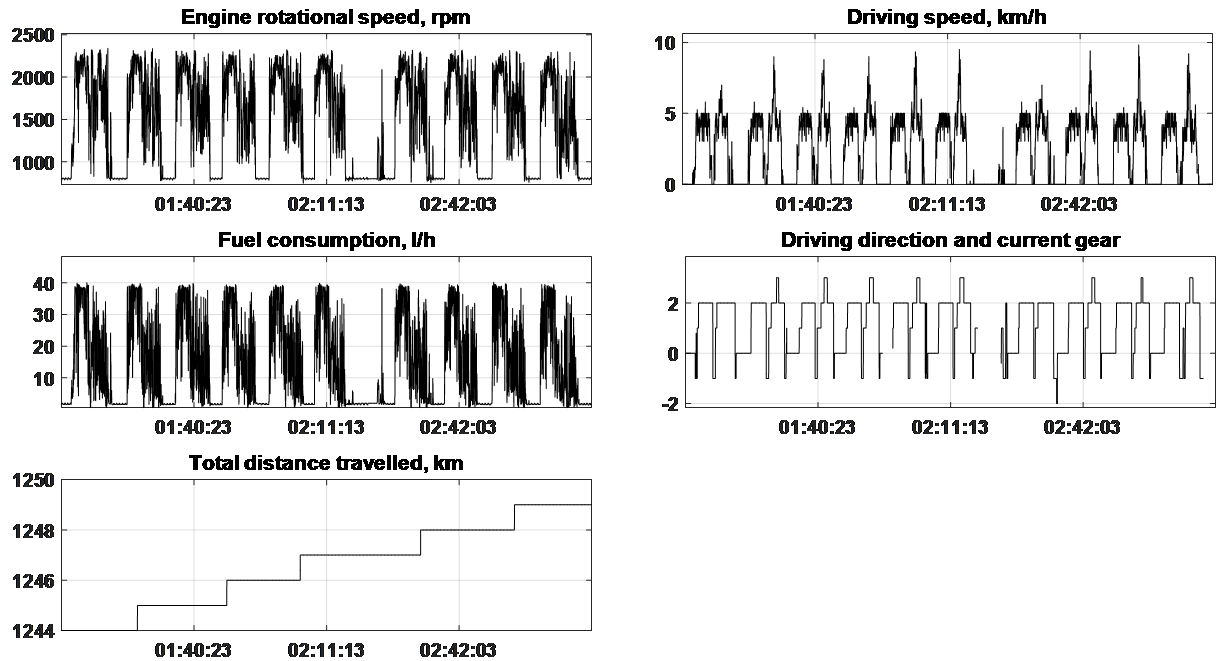
\includegraphics[width = 1\textwidth]{Wykresy/list_variables.png}
\caption{Key variables for efficiency assesment of haulars operation}
\label{fig: f1}
\end{figure}
As mentioned early haulers operation is not complex - machines are driving from point A to point B. As one can see in Fig. \ref{fig: f1} time series are characterised by cyclic variability, very similar in following haulage cycles. Assessment of their performance requires development of algorithm to identify each  operation regime of haulage (loading, haulage, unloading, return to mining face) by appropriate signals segmentation \cite{Lopatka,Polak2006,Stefaniak2015,Stefaniak2014,Wylomanska2014}. 
For haulers this task can seem to be very easy to solve. However, taking into account harsh and specific conditions in mining corridors, recognition of these regimes is hard to achieve using classical methods based on single variable and \emph{if-then-else} rules. Currently development of signals separation techniques leads to obtain components with a variable content regard to signal segmentation.
\section{Methodology for identification of haulage process}
\subsection{JADE-ICA algorithm}
Joint Approximation Diagonalization of Eigenmatrices (JADE) is one of several blind source separation (BSS) techniques from the family of Independent Component Analysis (ICA) algorithms \cite{Cardoso1999,Cardoso1996,Comon,Krishnaveni2005}. It exploits the fourth order moments in order to extract the source signals from mixed signals. Principle of operation of JADE is given as follows:
\begin{itemize}
\renewcommand{\labelitemi}{$\bullet$}
\item Set of input data \textbf{X} is provided in the form of M-by-N matrix of $M$ input vectors of the length $N$.
\item The whitening matrix \textbf{P} and the set of prewhitened data $\bm{Z = PX}$ are estimated.
\item The fourth cumulants of the whitened mixtures $\bm{\hat{Q}}_i^Z$ are computed. Their m most significant eigenvalues $\lambda_{i}$ and their corresponding matrices $V_{i}$ are determined. An estimate of the unitary matrix $\bm{R}$ is obtained by maximizing the criteria $\lambda_{i}$ $V_{i}$ by means of joint diagonalization. If $\lambda_{i}$ $V_{i}$ cannot be exactly jointly diagonalized, the maximization of the criteria defines a joint approximate diagonalization.
\item An orthogonal contrast is optimized by finding the rotation matrix $\bm{R}$ such that the cumulant matrices are as diagonal as possible, according to the equation:
$$
\mathbf{R}=arg\min_{R}\sum_{i}Off\left(\mathbf{R}^{T}\mathbf{\hat{Q}}_i^Z\mathbf{R}\right)
$$
\item The mixing matrix $\bm{A}$ is estimated as $\bm{\hat{A}=RP^{-1}}$ and the output components are estimated as matrix $\bm{\hat{S}=\hat{A}^{-1} X}$ of the same size as \textbf{X}.
\end{itemize}
\section{Application to the real data}
Based on visual inspection and physical meaning three variables were selected for the analysis as the most promising: engine rotational speed, fuel consumption and vehicle speed. Vectors were merged into 3-by-N matrix and provided to JADE algorithm, that returned 3-by-N matrix of output components.
First output feature includes sufficient information about haulage process and its variability. It ensures easy segmentation in the context of regime recognition. Hence, it has been selected for further analysis. Selection can be done automatically, because JADE in contrast to some other ICA algorithms (e.g. FastICA) always outputs resulting component vectors in the same order (see Fig. \ref{fig: f2}).\par
Features were then slightly smoothed using moving average with window length equal to 20. It allowed to obtain clearer signal with more visible trend of behavior (see Fig. \ref{fig: smooth}).\par
\begin{figure}[ht!]
\centering
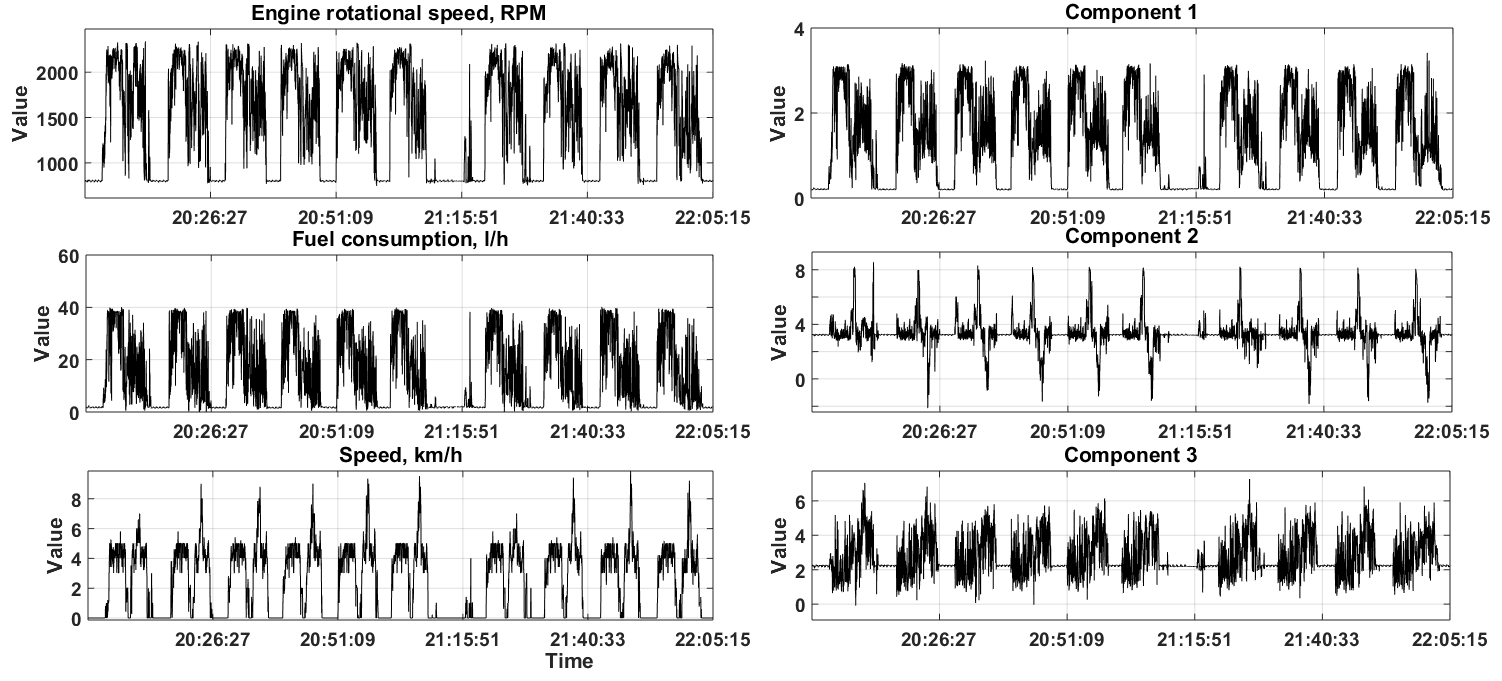
\includegraphics[width = 1\textwidth]{Wykresy/stats.png}
\caption{Input data (left panels) and smoothed independent components (right panels). Charts zoomed in time domain for better visibility.}
\label{fig: f2}
\vspace{-30pt}
\end{figure}
\begin{figure}[ht!]
\centering
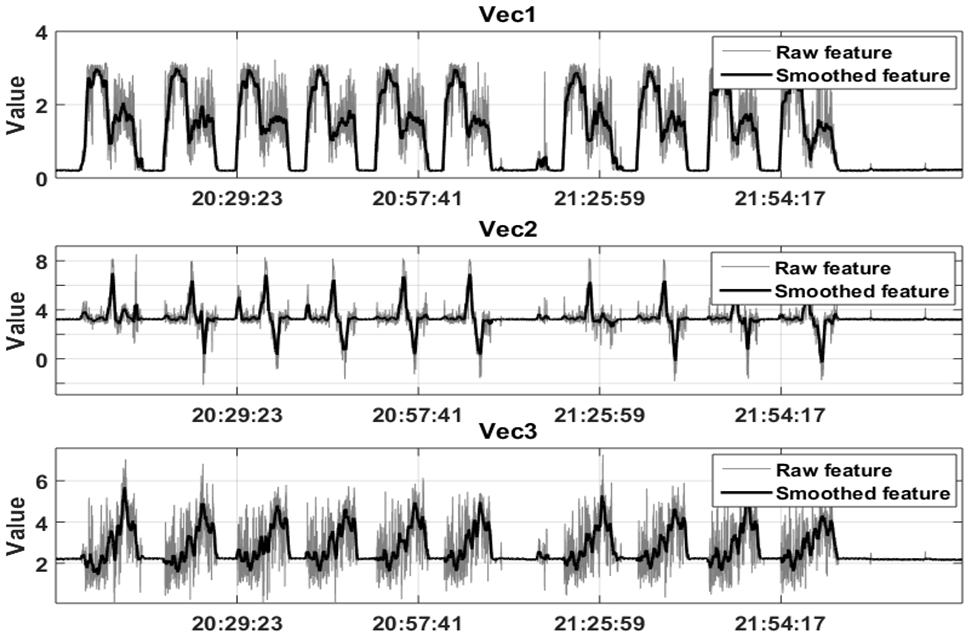
\includegraphics[width = 0.85\textwidth]{Wykresy/smooth.png}
\caption{Raw and smoothed output features}
\label{fig: smooth}
\end{figure}
In the next step we investigated expected subsets of values in the extracted feature. Smoothed kernel density estimate for selected component has been calculated (see Fig. \ref{fig: f3}), and its local minima define two thresholds that divide component values into three main regimes that are identified as:
\begin{itemize}
\renewcommand{\labelitemi}{$\bullet$}
\item loading of a cargo box,
\item driving to dumping point,
\item return from dumping point with empty cargo box.
\end{itemize}
\begin{figure}[ht!]
\vspace{-20pt}
\centering
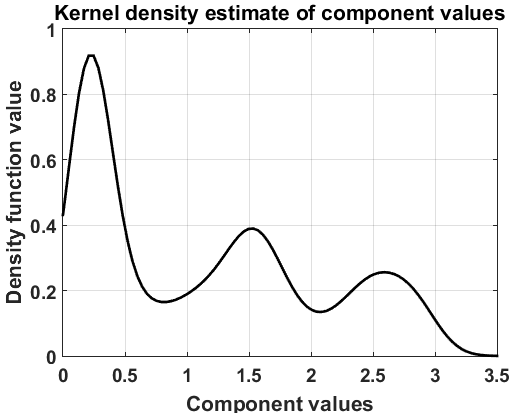
\includegraphics[width = 0.6\textwidth]{Wykresy/ksd.png}
\caption{Smoothed kernel density estimate of the selected component no. 1}
\label{fig: f3}
\end{figure}
We can make an assumption here, based on visual inspection of input data and output components, that first component selected for further analysis is connected to vaguely stated "machine operational load", since it is structurally mostly similar to engine speed and fuel consumption. We can then easily identify mentioned regimes:
\begin{figure}[ht!]
\centering
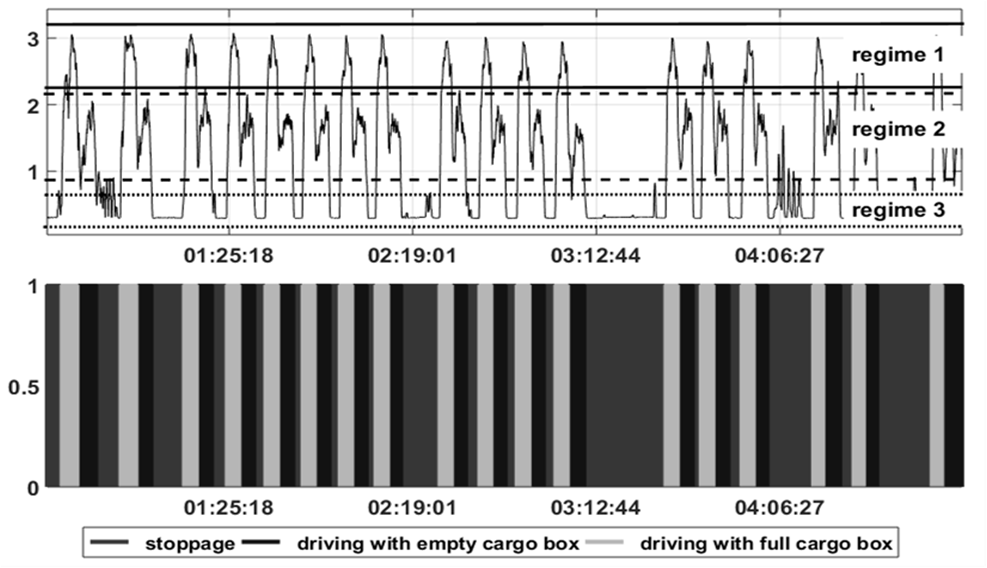
\includegraphics[width = 0.9\textwidth]{Wykresy/2.png}
\caption{Segmented component signal}
\label{fig: f4}
\end{figure}
\begin{figure}[ht!]
\centering
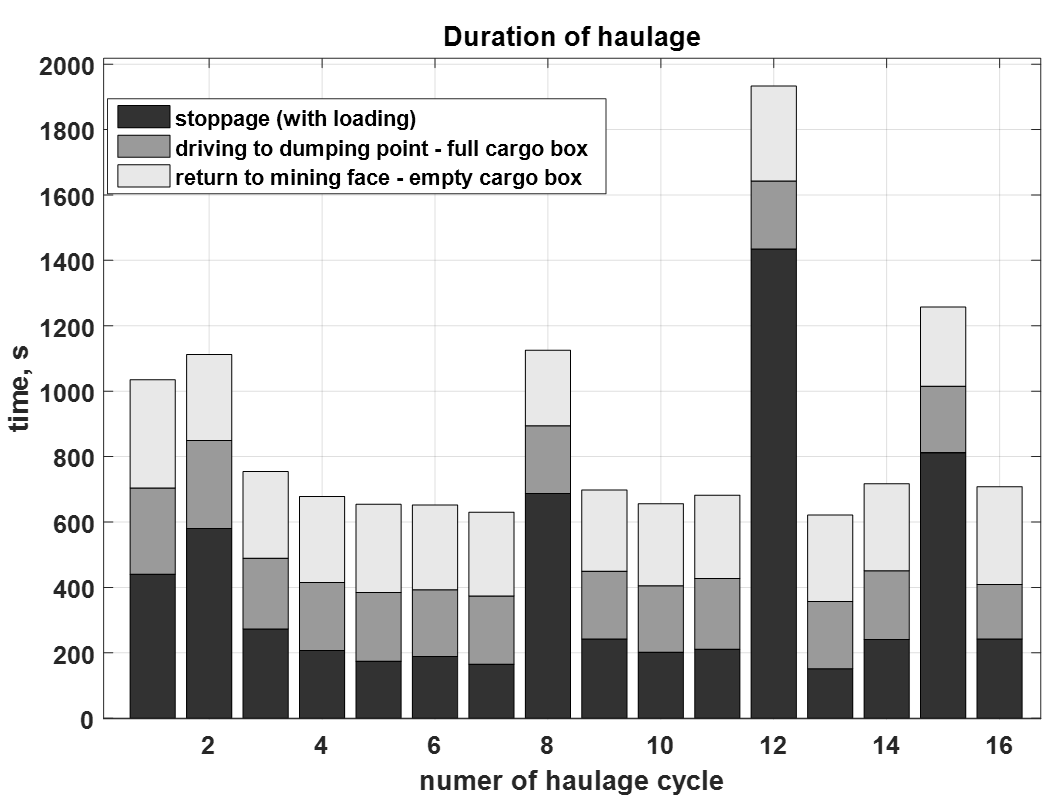
\includegraphics[width = 0.9\textwidth]{Wykresy/staty_czasy.png}
\caption{Duration of particular partial operations of haulage cycles from single shift}
\label{fig: f5}
\end{figure}
\begin{itemize}
\renewcommand{\labelitemi}{$\bullet$}
\item \textbf{Loading of a cargo box} will take the lowest values. Machine is standing still and its cargo box is being loaded, engine load is the lowest.
\item \textbf{Driving to dumping screen} will take the highest values. Cargo bucket is full and machine is driving under load.
\item \textbf{Returning from the screen} will take medium values. Machine is driving, but with empty cargo bucket, which results in moderate load.
\end{itemize}
Signal of this component is then segmented according to obtained regimes of values (see Fig. \ref{fig: f4}). At the end of segmentation, data is post-processed just to eliminate very short improperly detected regimes originating from unexpected spikes in the signal, that were present because of the way that decomposition into independent components occurred.\par
As Fig. \ref{fig: f4} shows, regimes are identified in very clear and correct way, that can allow for further statistical analysis related to process optimisation see Fig \ref{fig: f5}.
\section{Summary}
Segmentation of operational data is just a pre-processing stage for further analysis. Extraction of cycles with its partial operations might allow to analyse performance of machines. In haulers case, identification of operational regimes and working cycles leads to constructing the algorithms like e.g. counting cycles in relation to time, analysis of regimes and cycles duration, detection of unexpected stoppages in the workflow etc. (see Fig \ref{fig: f5}). Such indicators might give many information about realization of production in mining face and allow to support mining staff in context of better work organization.
In this paper we present signal segmentation method based on independent component decomposition of hauler operational data. Results show that feature extraction methods can create good foundation for parameterization before applying segmentation procedures.

 \begin{thebibliography}{}
%
% and use \bibitem to create references. Consult the Instructions
% for authors for reference list style.
%

\bibitem{Cardoso1999} Cardoso J.F., \emph{High-order contrasts for independent component analysis}, 1999, Neural Computation. Vol. 11, No 1, pp. 157-192.

\bibitem{Cardoso1996} Cardoso J.F., Bose S., Friedlander B., \emph{On optima source separation based on second and fourth order cumulants}, 1996, Statistical Signal and Array Processing.8th IEEE Signal Processing Workshop in Corfu. pp. 198-201.

\bibitem{Comon} Comon P., Jutten Ch., \emph{Handbook of blind source separation: Independent Component Analysis and Applications}, 2010, Elsevier, ISBN: 978-0-12-374726-6.

\bibitem{Krishnaveni2005} Krishnaveni V., Jayaraman S., Manoj Kumar P. M., Shivakumar K., Ramadoss K., \emph{Comparison of Independent Component Analysis algorithms for removal of ocular artifacts from electroencephalogram}, 2005, Measurement Science Review. Vol. 5, No 2, pp. 67-78.

\bibitem{Lopatka} Lopatka  M.,  Laplanche  C.,  Adam  O.,  Motsch  J.-F.,  Zarzycki  J.,  \emph{Non-stationary  time-series segmentation based on the Schur prediction error analysis},  2005, 13th Workshop on Statistical Signal Processing, pp. 251- 256, DOI: 10.1109/SSP.2005.1628601.

\bibitem{Polak2006} Polak M., Stefaniak P.K., Zimroz R., Wylomanska A., Sliwinski P., Andrzejewski M., \emph{Identification of loading process based on hydraulic pressure signal}, 2016, The conference proceedings of 16th International multidisciplinary scientific geoconference SGEM 2016. pp. 459-466.

\bibitem{Stefaniak2015} Stefaniak P.K., Zimroz R., Obuchowski J., Sliwinski P., Andrzejewski M., \emph{An effectiveness indicator for a mining loader based on the pressure signal measured at a bucket's hydraulic cylinder}, 2015, Procedia Earth and Planetary Science. Vol. 15, pp. 797-805.

\bibitem{Stefaniak2014} Stefaniak P.K., Zimroz R., Sliwinski P., Andrzejewski M., Wylomanska A.,  \emph{Multidimensional signal analysis for technical condition, operation and performance understanding of heavy duty mining machines}, 2016, Advances in Condition Monitoring of Machinery in Non-Stationary Operations. Applied Condition Monitoring. Vol. 4, pp. 197-210.

\bibitem{Wylomanska2014} Wylomanska A., Zimroz R., \emph{Signal segmentation for operational regimes detection of heavy duty mining mobile machines- a statistical approach}, 2014 Diagnostyka. Vol. 15 No 2, pp. 33-42.




\end{thebibliography}

\end{document}
% end of file template.tex
